 \documentclass{article}
\usepackage{graphicx}% http://ctan.org/pkg/graphicx
\usepackage{array}% http://ctan.org/pkg/array
\begin{document}

\begin{table}[h!]
  \centering
  \begin{tabular}{ | m{5 cm} | m{3cm} | m{3cm} | }
    \hline
   Result &  min and max & mean and standard deviation \\ \hline
    \begin{minipage}{.3\textwidth}
      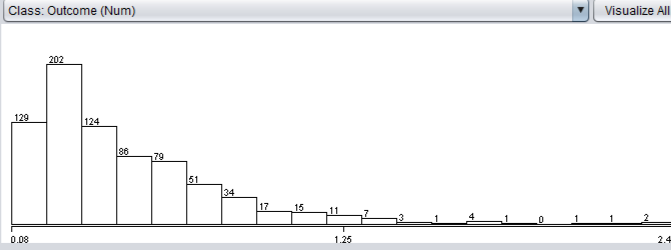
\includegraphics[width=\linewidth, height=60mm]{diabetes/diabetes.png}
    \end{minipage}
    &
    %\begin{minipage}[t]{5cm}
      \begin{itemize}
        \item  min is 0.078
        \item max is 2.42
          
      \end{itemize}
    %\end{minipage}
    & 
    %\begin{minipage}{5cm}
      \begin{itemize}
        \item  mean is 0.472
        \item  standard deviation is 0.331  
          
      \end{itemize}
    %\end{minipage}
    \\ \hline
  \end{tabular}
  \caption{ diabetesPedigreeFunction}\label{tbl:myLboro}
\end{table}
\begin{table}[h!]
  \centering
  \begin{tabular}{ | m{5 cm} | m{3cm} | m{3cm} | }
    \hline
   Result &  min and max & mean and standard deviation \\ \hline
    \begin{minipage}{.3\textwidth}
      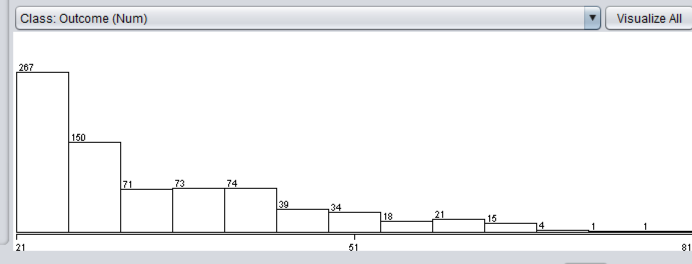
\includegraphics[width=\linewidth, height=60mm]{age.png}
    \end{minipage}
    &
    %\begin{minipage}[t]{5cm}
      \begin{itemize}
        \item  min is 21
        \item max is 81
          
      \end{itemize}
    %\end{minipage}
    & 
    %\begin{minipage}{5cm}
      \begin{itemize}
        \item  mean is 33.241
        \item  standard deviation is 11.76 
          
      \end{itemize}
    %\end{minipage}
    \\ \hline
  \end{tabular}
  \caption{ Age}\label{tbl:myLboro}
\end{table}
\begin{table}[h!]
  \centering
  \begin{tabular}{ | m{5 cm} | m{3cm} | m{3cm} | }
    \hline
   Result &  min and max & mean and standard deviation \\ \hline
    \begin{minipage}{.3\textwidth}
      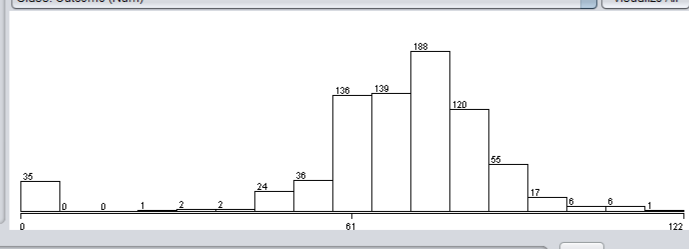
\includegraphics[width=\linewidth, height=60mm]{blood pressure.png}
    \end{minipage}
    &
    %\begin{minipage}[t]{5cm}
      \begin{itemize}
        \item  min is 0
        \item max is 122
          
      \end{itemize}
    %\end{minipage}
    & 
    %\begin{minipage}{5cm}
      \begin{itemize}
        \item  mean is 69.105
        \item  standard deviation is 19.356  
          
      \end{itemize}
    %\end{minipage}
    \\ \hline
  \end{tabular}
  \caption{ BLOOD Pressure}\label{tbl:myLboro}
\end{table}
\begin{table}[h!]
  \centering
  \begin{tabular}{ | m{5 cm} | m{3cm} | m{3cm} | }
    \hline
   Result &  min and max & mean and standard deviation \\ \hline
    \begin{minipage}{.3\textwidth}
      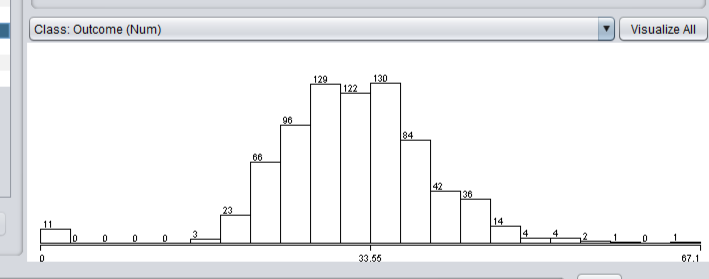
\includegraphics[width=\linewidth, height=60mm]{BMI.png}
    \end{minipage}
    &
    %\begin{minipage}[t]{5cm}
      \begin{itemize}
        \item  min is 0
        \item max is 67.1
          
      \end{itemize}
    %\end{minipage}
    & 
    %\begin{minipage}{5cm}
      \begin{itemize}
        \item  mean is 31.993
        \item  standard deviation is 7.884  
          
      \end{itemize}
    %\end{minipage}
    \\ \hline
  \end{tabular}
  \caption{ BMI }\label{tbl:myLboro}
\end{table}
\begin{table}[h!]
  \centering
  \begin{tabular}{ | m{5 cm} | m{3cm} | m{3cm} | }
    \hline
   Result &  min and max & mean and standard deviation \\ \hline
    \begin{minipage}{.3\textwidth}
      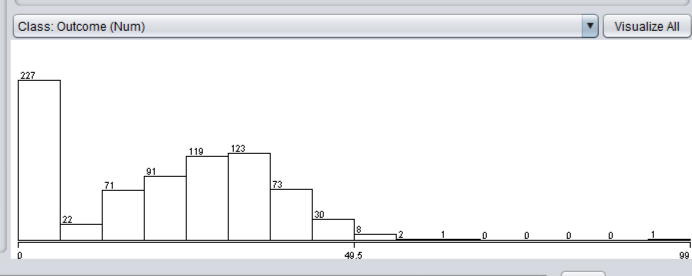
\includegraphics[width=\linewidth, height=60mm]{skin thickness.png}
    \end{minipage}
    &
    %\begin{minipage}[t]{5cm}
      \begin{itemize}
        \item  min is 0
        \item max is 99
          
      \end{itemize}
    %\end{minipage}
    & 
    %\begin{minipage}{5cm}
      \begin{itemize}
        \item  mean is 20.536
        \item  standard deviation is 15.952 
          
      \end{itemize}
    %\end{minipage}
    \\ \hline
  \end{tabular}
  \caption{ skin thickness }\label{tbl:myLboro}
\end{table}
\begin{table}[h!]
  \centering
  \begin{tabular}{ | m{5 cm} | m{3cm} | m{3cm} | }
    \hline
   Result &  min and max & mean and standard deviation \\ \hline
    \begin{minipage}{.3\textwidth}
      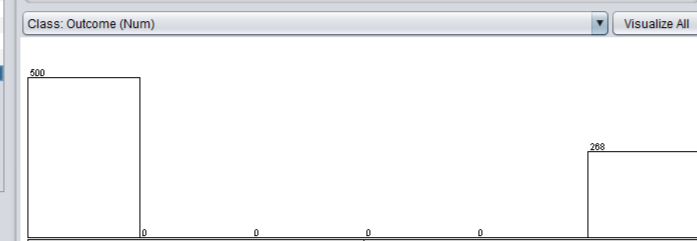
\includegraphics[width=\linewidth, height=60mm]{outcome.png}
    \end{minipage}
    &
    %\begin{minipage}[t]{5cm}
      \begin{itemize}
        \item  min is 0
        \item max is 1
          
      \end{itemize}
    %\end{minipage}
    & 
    %\begin{minipage}{5cm}
      \begin{itemize}
        \item  mean is 0.349
        \item  standard deviation is 0.477  
          
      \end{itemize}
    %\end{minipage}
    \\ \hline
  \end{tabular}
  \caption{ outcome }\label{tbl:myLboro}
\end{table}
\begin{table}[h!]
  \centering
  \begin{tabular}{ | m{5 cm} | m{3cm} | m{3cm} | }
    \hline
   Result &  min and max & mean and standard deviation \\ \hline
    \begin{minipage}{.3\textwidth}
      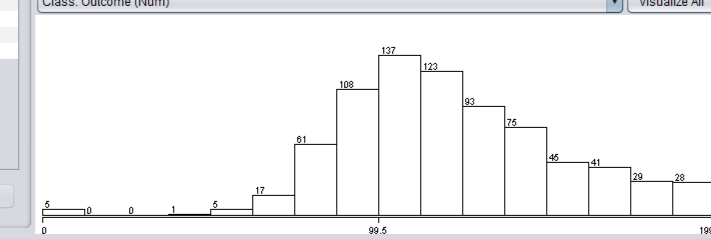
\includegraphics[width=\linewidth, height=60mm]{glucose.png}
    \end{minipage}
    &
    %\begin{minipage}[t]{5cm}
      \begin{itemize}
        \item  min is 0
        \item max is 67.1
          
      \end{itemize}
    %\end{minipage}
    & 
    %\begin{minipage}{5cm}
      \begin{itemize}
        \item  mean is 12.895
        \item  standard deviation is 31.9
          
      \end{itemize}
    %\end{minipage}
    \\ \hline
  \end{tabular}
  \caption{ glucose }\label{tbl:myLboro}
\end{table}
\begin{table}[h!]
  \centering
  \begin{tabular}{ | m{5 cm} | m{3cm} | m{3cm} | }
    \hline
   Result &  min and max & mean and standard deviation \\ \hline
    \begin{minipage}{.3\textwidth}
      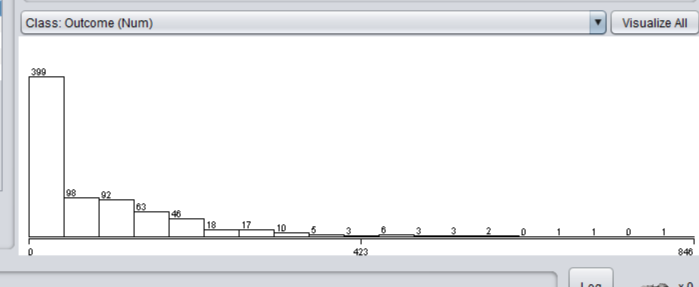
\includegraphics[width=\linewidth, height=60mm]{insulin.png}
    \end{minipage}
    &
    %\begin{minipage}[t]{5cm}
      \begin{itemize}
        \item  min is 0
        \item max is 846
          
      \end{itemize}
    %\end{minipage}
    & 
    %\begin{minipage}{5cm}
      \begin{itemize}
        \item  mean is 79.799
        \item  standard deviation is 115.244
          
      \end{itemize}
    %\end{minipage}
    \\ \hline
  \end{tabular}
  \caption{ Insulin }\label{tbl:myLboro}
\end{table}

\end{document}